%%%%%%%%%%%%%%%%%%%%%%%%%%%%%%%%%%%%%%%%%%%%%%%%%%%%%%%%%%%%%%%%%%%%%%%%%%%%
%% Author template for INFORMS Journal on Data Science (ijds) [interim solution; new styles under construction]
%% Mirko Janc, Ph.D., INFORMS, mirko.janc@informs.org
%% ver. 0.91, March 2015 - updated November 2020 by Matthew Walls, matthew.walls@informs.org
%% Adapted for rticles by Rob J Hyndman Rob.Hyndman@monash.edu. Dec 2021
%%%%%%%%%%%%%%%%%%%%%%%%%%%%%%%%%%%%%%%%%%%%%%%%%%%%%%%%%%%%%%%%%%%%%%%%%%%%
\documentclass[,,nonblindrev]{informs}

\OneAndAHalfSpacedXI
%%\OneAndAHalfSpacedXII % Current default line spacing
%%\DoubleSpacedXII
%%\DoubleSpacedXI

%% BEGIN MY ADDITIONS %%
\usepackage{hyperref}

% tightlist command for lists without linebreak
\providecommand{\tightlist}{%
  \setlength{\itemsep}{0pt}\setlength{\parskip}{0pt}}



\usepackage{booktabs}
\usepackage{siunitx}
\usepackage{tablefootnote}
\usepackage{longtable}
\usepackage{threeparttable}
\usepackage{natbib}

%% END MY ADDITIONS %%


% Natbib setup for author-year style
\usepackage{natbib}
 \bibpunct[, ]{(}{)}{,}{a}{}{,}%
 \def\bibfont{\small}%
 \def\bibsep{\smallskipamount}%
 \def\bibhang{24pt}%
 \def\newblock{\ }%
 \def\BIBand{and}%


%% Setup of theorem styles. Outcomment only one.
%% Preferred default is the first option.
\TheoremsNumberedThrough     % Preferred (Theorem 1, Lemma 1, Theorem 2)
%\TheoremsNumberedByChapter  % (Theorem 1.1, Lema 1.1, Theorem 1.2)
\ECRepeatTheorems

%% Setup of the equation numbering system. Outcomment only one.
%% Preferred default is the first option.
\EquationsNumberedThrough    % Default: (1), (2), ...
%\EquationsNumberedBySection % (1.1), (1.2), ...

% For new submissions, leave this number blank.
% For revisions, input the manuscript number assigned by the on-line
% system along with a suffix ".Rx" where x is the revision number.
\MANUSCRIPTNO{}

%%%%%%%%%%%%%%%%
\begin{document}
%%%%%%%%%%%%%%%%

% Outcomment only when entries are known. Otherwise leave as is and
%   default values will be used.
%\setcounter{page}{1}
%\VOLUME{00}%
%\NO{0}%
%\MONTH{Xxxxx}% (month or a similar seasonal id)
%\YEAR{0000}% e.g., 2005
%\FIRSTPAGE{000}%
%\LASTPAGE{000}%
%\SHORTYEAR{00}% shortened year (two-digit)
%\ISSUE{0000} %
%\LONGFIRSTPAGE{0001} %
%\DOI{10.1287/xxxx.0000.0000}%

% Author's names for the running heads
% Sample depending on the number of authors;
\RUNAUTHOR{%
Jameson, Saghafian, Huckman
 and Hodgson
}
% \RUNAUTHOR{Jones and Wilson}
% \RUNAUTHOR{Jones, Miller, and Wilson}
% \RUNAUTHOR{Jones et al.} % for four or more authors
% Enter authors following the given pattern:
%\RUNAUTHOR{}

\RUNTITLE{To Batch or Not to Batch: Sequential vs.~Batched Testing
Strategies in the ED}

\TITLE{To Batch or Not to Batch: Sequential vs.~Batched Testing
Strategies in the ED}

\ARTICLEAUTHORS{%
\AUTHOR{Jacob Jameson}
\AFF{Interfaculty Initiative in Health Policy, Harvard
University, \EMAIL{\href{mailto:jacobjameson@g.harvard.edu}{\nolinkurl{jacobjameson@g.harvard.edu}}}}

\AUTHOR{Soroush Saghafian}
\AFF{Kennedy School of Government, Harvard
University, \EMAIL{\href{mailto:soroush_saghafian@hks.harvard.edu}{\nolinkurl{soroush\_saghafian@hks.harvard.edu}}}}

\AUTHOR{Robert Huckman}
\AFF{Harvard Business
School, \EMAIL{\href{mailto:rhuckman@hbs.edu}{\nolinkurl{rhuckman@hbs.edu}}}}

\AUTHOR{Nicole Hodgson}
\AFF{Mayo
Clinic, \EMAIL{\href{mailto:Hodgson.Nicole@mayo.edu}{\nolinkurl{Hodgson.Nicole@mayo.edu}}}}

%
}

\ABSTRACT{This paper focuses on analyzing sequential versus batched
testing strategies in an emergency department (ED) at Mayo Clinic
Arizona, with respect to their associations impacts on patient length of
stay, hospital readmission, and healthcare resource utilization. A
theoretical model was developed and tested to identify patient and
hospital features that may influence the decision to batch or
sequentially order tests, such as patient complexity, physician
experience, occupancy level and complexity. Finally, we performed
retrospective analysis of ED operational data to investigate the impact
of batching on our key outcomes. The overall result was that batch
ordering tests was associated with greater patient length of stay and
resource utilization, even when we control for variation in patient
complexity, physician experience, and hospital occupancy.}

\KEYWORDS{Emergency Department, Operational Effeciency, Diagnostic
Testing}

\maketitle


\hypertarget{sec:1}{%
\section{Introduction}\label{sec:1}}

Healthcare delivery, particularly in the emergency department (ED), is a
delicate balance that involves ensuring optimal patient outcomes while
optimizing resource utilization. Achieving these twin goals requires
timely and accurate diagnosis, which in turn enables prompt and
appropriate treatment, consequently improving patient prognosis and
reducing the likelihood of adverse events. Furthermore, efficient
patient discharge from the ED can help alleviate overcrowding, a severe
issue with potential consequences including higher complication rates
and increased mortality \citet{bernstein2009}.

One important factor that can impact the speed and effectiveness of
diagnosis in the ED is the availability and performance of diagnostic
tests \citet{naseim2015}. A variety of diagnostic tests are used in the
ED, including laboratory tests, imaging studies, and specialized tests
such as electrocardiograms (ECGs) and point-of-care (POC) testing. These
tests can provide valuable information about a patient's condition and
help to guide treatment decisions.

A critical question in this context pertains to whether physicians in
the ED should batch order diagnostic tests or order them sequentially.
This decision essentially represents a tradeoff between reducing patient
length of stay and risk of over-testing. Over-testing, or performing
unnecessary tests, can lead to increased costs, unnecessary patient
anxiety, and potential harm from follow-up of false-positive results
\citet{koch2018}. Conversely, keeping a patient for an extended time to
perform all possible tests could lead to ED overcrowding, an issue
associated with severe consequences, as mentioned earlier. Instead, what
is needed is a reasonable balance between the number of diagnostic tests
performed and the total time the patient is kept in the ED before either
being admitted or discharged. Several studies have demonstrated that
optimizing the ED patient flow process can result in significant
improvements \citet{saghafian2015}, however, research surrounding test
ordering strategies to improve the patient flow processes remains
limited.

In this paper, we use data from over 41,000 patient visits to the ED
that occur during our study period to quantify the benefits and
consequences of batching versus sequentially ordering diagnostic tests
on patient length of stay, re-admission, and resource utilization. Our
empirical strategy exploits random assignment of patients to ED
physicians who differ in their propensity to batch-order diagnostic
tests. When patients arrive at the ED, they are assigned to a physician
based on availability, with no discretion on either side. Thus, patients
who arrive at the ED at similar times are randomly assigned to
physicians who vary in their willingness to batch order diagnostic
tests. We measure physician tendency to batch using a leave-out,
residualized measure based on all other patients the physician has seen
in the ED in the study period. The tendency measure strongly predicts
the ED test batch outcome but is uncorrelated with patient and ED visit
characteristics.

We start by evaluating the reduced-form effects of ED provider batch
ordering tendency on downstream patient outcomes and turnaround time. We
find that practice variation as captured by physician batch-ordering
tendency has large and significant consequences. Being treated by a
provider in the top decile of the leniency distribution, compared to
being treated by someone in the bottom decile {[}INSERT RESULTS{]}.

Because of the institutional features of the ED, our research design
closely approximates an RCT that assigns patients to batch-ordering or
sequential-ordering arm. In the ED, patients have no discretion over
choosing providers, and in our specific ED, physicians have discretion
over choosing patients, alleviating major selection issues present in
other health care settings. Furthermore, physicians exhibit wide
variation in practice behavior in batch ordering, even within the same
hospital, while following the same guidelines. Finally,
patient-physician interactions in the ED are typically well documented,
short, and one-off, constraining physician decision-making to a more
limited, better-observed choice set than present in settings such as
specialty or primary care.

In sum, exploiting practice variation in ED settings shuts down other
(but not all) potential channels besides test batching that are present
in other settings, determine length of stay, and impact patient
outcomes. This approach allows us to move closer to identifying the
causal impact of batch-ordering diagnostic tests on patient outcomes and
hospital effeciency. It is important to note that this paper studies the
impact of an batch-ordering through a batching decision requiring
clinical judgment (within practice norms) rather than through specific
hospital policies, differences in adherence to clinical practice
guidelines, or substandard care.

The remainder of this paper is structured as follows. The next section
describes the data source and outlines our baseline sample. The
empirical strategy and its accompanying identifying assumptions are laid
out in Section II. Section III presents the results. Section IV draws
implications for batch-ordering policies. The last section concludes.

\hypertarget{sec:2}{%
\section{Data and Definitions}\label{sec:2}}

Our analytical lens is focused on the Emergency Department at the Mayo
Clinic of Arizona, a distinguished tertiary care establishment. During
our study's timeframe, the ED recorded an annual visitation of
approximately 41,000 patients. The department is singularly staffed by
board-eligible or board-certified emergency physicians, abstaining from
the services of nurse practitioners or physician assistants. A notable
observation was that residents in rotation oversaw a low fraction,
roughly 10\%, of the patient volume. Comprehensive patient data,
encompassing demographics, chief complaints, vital signs, emergency
severity, length of stay, and resource utilization metrics, were
meticulously logged during the study period.

\hypertarget{sample-construction}{%
\subsection{Sample Construction}\label{sample-construction}}

We identified three distinct forms of test batching:

\begin{itemize}
\item
  Lab/Image Batch: The first test ordered for a patient was either an
  imaging or lab test (CT scan, X-ray, Ultrasound, Lab), followed by an
  additional imaging or lab test order within 5 minutes.
\item
  Image/Image Batch: The first test ordered for a patient was an imaging
  test (CT scan, X-ray, Ultrasound), followed by an additional imaging
  test order within 5 minutes.
\item
  Any Batch: This refers to instances where either a Lab/Image Batch or
  an Image/Image Batch occurred.
\end{itemize}

We conducted a sensitivity analysis for this definition, documented in
Appendix 2. Table 1 highlights the considerable variation in patient
complexity between those who had their tests batch ordered versus those
where tests were ordered sequentially.

\hypertarget{statistics}{%
\subsection{Statistics}\label{statistics}}

Table 1 provides a comprehensive breakdown of the patient encounters
involving diagnostic tests ordered either individually (Sequential) or
as part of a group (Batch) during an ED encounter from our baseline
sample. Around 43\% of patient encounters involved diagnostic tests
ordered as part of a batch, the majority of which (60\%) included two
tests.

Differences were noted between the two cohorts. Patients who had batched
tests ordered tended to have a longer ED length of stay, a lower
Emergency Severity Index (ESI), and were generally older than those who
had their tests ordered individually. Patients in the batch order group
were also more likely to present with symptoms at triage, including
tachycardia, tachypnea, fever, and hypotension. A deeper dive into the
ESI data reveals a higher proportion of patients with more urgent
conditions (ESI 1 and 2) in the batched group than in the sequential
group. This finding might be indicative of the complexity and severity
of the conditions of patients who necessitate batch testing.

Age distributions between the two groups demonstrate a greater
proportion of patients aged 65 and above in the batch group, suggesting
that older patients are more likely to have multiple tests ordered at
once, possibly due to the presence of multiple comorbidities. The
batched group showed a longer average ED length of stay compared to the
sequential group. This extended stay may be reflective of the additional
time required to conduct and evaluate the results of multiple tests.
Symptoms presentation at triage also differed between the two groups,
with the batched group being more likely to present with tachypnea,
fever, and hypotension. However, tachycardia was found to be similar
across both groups.

\begin{table}[htbp]
\centering
\tiny
\caption{Summary Statistics for Sequential vs. Batched Test Groups}
\begin{tabular}{lcccc}
\hline
Variable & \multicolumn{1}{c}{Overall Visits, N = 41,197\textsuperscript{1}} & \multicolumn{1}{c}{Sequential Arm, N = 23,4331} & \multicolumn{1}{c}{Batching Arm, N = 17,7641} & \multicolumn{1}{c}{p-value\textsuperscript{2}} \\
\hline
\textbf{ESI} & & & & $<$0.001 \\
\hspace{0.5cm} 1 & 474 (1.2\%) & 130 (0.6\%) & 344 (1.9\%) & \\
\hspace{0.5cm} 2 & 13,911 (34\%) & 6,502 (28\%) & 7,409 (42\%) & \\
\hspace{0.5cm} 3 & 23,655 (57\%) & 14,350 (61\%) & 9,305 (52\%) & \\
\hspace{0.5cm} 4 & 3,123 (7.6\%) & 2,422 (10\%) & 701 (3.9\%) & \\
\hspace{0.5cm} 5 & 34 ($<$0.1\%) & 29 (0.1\%) & 5 ($<$0.1\%) & \\
\hline
\textbf{Age} & & & & $<$0.001 \\
\hspace{0.5cm} $<$20 & 790 (1.9\%) & 605 (2.6\%) & 185 (1.0\%) & \\
\hspace{0.5cm} 20-45 & 9,412 (23\%) & 6,242 (27\%) & 3,170 (18\%) & \\
\hspace{0.5cm} 45-65 & 12,826 (31\%) & 7,393 (32\%) & 5,433 (31\%) & \\
\hspace{0.5cm} 65+ & 18,169 (44\%) & 9,193 (39\%) & 8,976 (51\%) & \\
\hline
\textbf{ED LOS} & & & & $<$0.001 \\
\hspace{0.5cm} Mean (SD) & 270 (382) & 258 (177) & 286 (545) & \\
\hline
\textbf{72hr Return} & 1,482 (3.6\%) & 957 (4.1\%) & 525 (3.0\%) & $<$0.001 \\
\hline
\textbf{Number of Tests} & & & & $<$0.001 \\
\hspace{0.5cm} 1 & 12,961 (31\%) & 11,937 (51\%) & 1,024 (5.8\%) & \\
\hspace{0.5cm} 2 & 19,112 (46\%) & 8,457 (36\%) & 10,655 (60\%) & \\
\hspace{0.5cm} 3 & 7,688 (19\%) & 2,581 (11\%) & 5,107 (29\%) & \\
\hspace{0.5cm} 4 & 1,342 (3.3\%) & 432 (1.8\%) & 910 (5.1\%) & \\
\hspace{0.5cm} 5 & 94 (0.2\%) & 26 (0.1\%) & 68 (0.4\%) & \\
\hline
\textbf{Disposition} & & & & $<$0.001 \\
\hspace{0.5cm} Discharge & 25,302 (61\%) & 15,922 (68\%) & 9,380 (53\%) & \\
\hspace{0.5cm} Admit & 9,097 (22\%) & 4,209 (18\%) & 4,888 (28\%) & \\
\hspace{0.5cm} Other & 6,798 (17\%) & 3,302 (14\%) & 3,496 (20\%) & \\
\hline
\textbf{Tachycardic} & 8,115 (20\%) & 4,562 (19\%) & 3,553 (20\%) & 0.18 \\
\hline
\textbf{Tachypneic} & 3,822 (9.3\%) & 1,669 (7.1\%) & 2,153 (12\%) & $<$0.001 \\
\hline
\textbf{Febrile} & 969 (2.4\%) & 353 (1.5\%) & 616 (3.5\%) & $<$0.001 \\
\hline
\textbf{Hypotensive} & 651 (1.6\%) & 305 (1.3\%) & 346 (1.9\%) & $<$0.001 \\
\hline
\textbf{Gender} & & & & $<$0.001 \\
\hspace{0.5cm} Female & 22,105 (54\%) & 12,986 (55\%) & 9,119 (51\%) & \\
\hspace{0.5cm} Male & 19,092 (46\%) & 10,447 (45\%) & 8,645 (49\%) & \\
\hline
\textbf{Race} & & & & $<$0.001 \\
\hspace{0.5cm} White & 36,554 (89\%) & 20,665 (88\%) & 15,889 (89\%) & \\
\hspace{0.5cm} Black & 1,682 (4.1\%) & 974 (4.2\%) & 708 (4.0\%) & \\
\hspace{0.5cm} Asian & 1,217 (3.0\%) & 710 (3.0\%) & 507 (2.9\%) & \\
\hspace{0.5cm} Other & 737 (1.8\%) & 449 (1.9\%) & 288 (1.6\%) & \\
\hspace{0.5cm} Native & 538 (1.3\%) & 340 (1.5\%) & 198 (1.1\%) & \\
\hspace{0.5cm} Unknown & 469 (1.1\%) & 295 (1.3\%) & 174 (1.0\%) & \\
\hline
\hline
\multicolumn{5}{l}{\textsuperscript{1} n (\%)} \\
\multicolumn{5}{l}{\textsuperscript{2} Pearson's Chi-squared test; Welch Two Sample t-test} \\
\end{tabular}
\end{table}

\begin{figure}
\centering
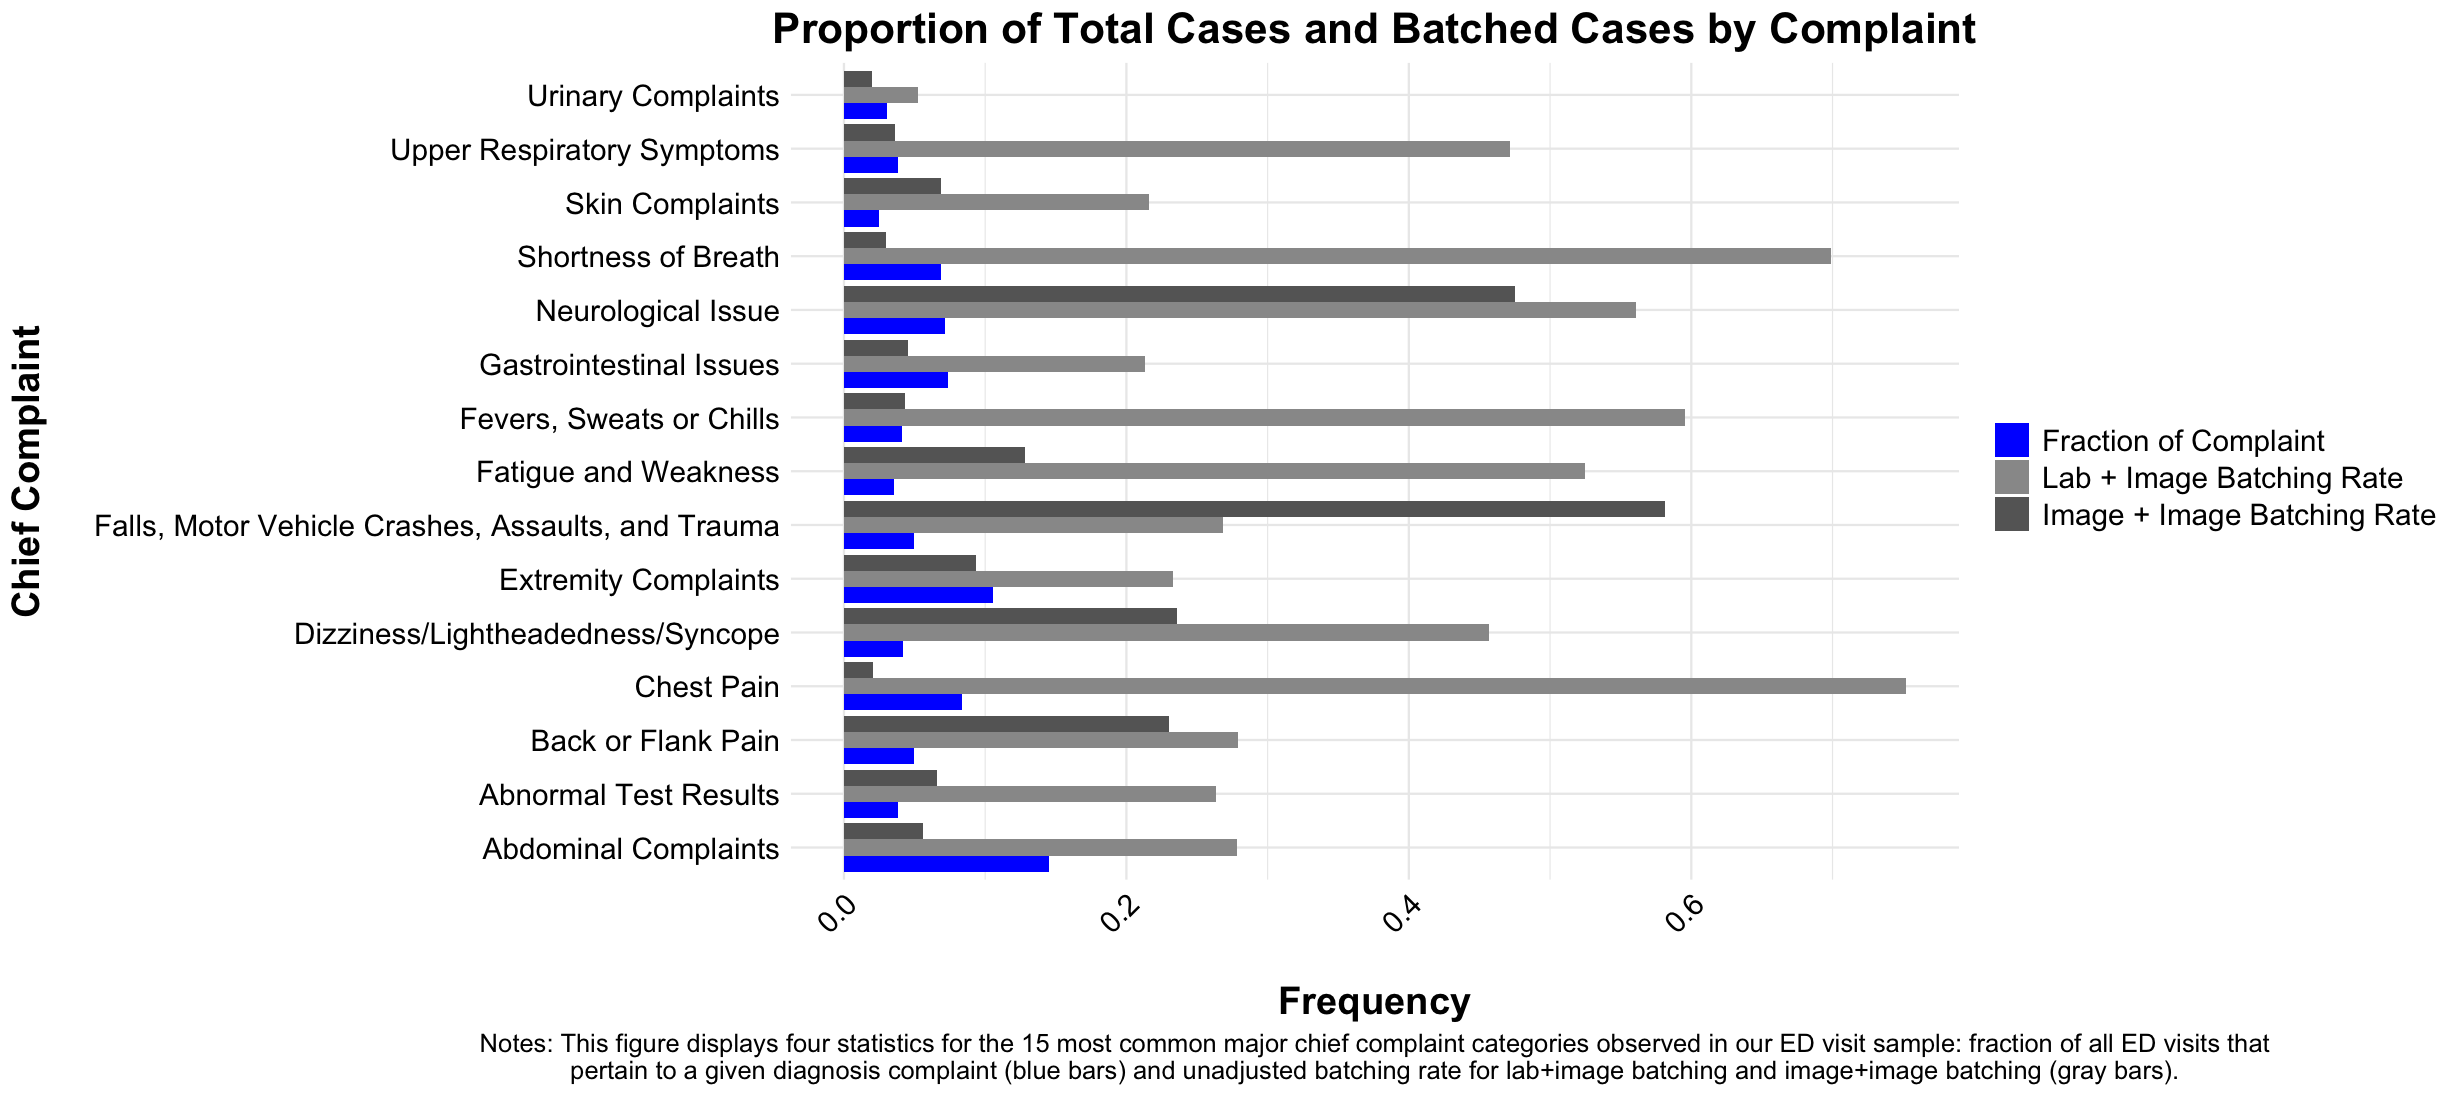
\includegraphics[width=\textwidth,height=0.3\textheight]{../Manuscript/figures/fig1.png}
\caption{Frequency of Sample Cases and Batches}
\end{figure}

\hypertarget{institutional-details-on-patient-physician-assignment}{%
\subsection{Institutional Details on Patient-Physician
Assignment}\label{institutional-details-on-patient-physician-assignment}}

Contrary to most healthcare settings where patients exhibit choice, they
are predominantly passive in their physician assignment in the ED. In
most EDs, however, physicians have discretion in picking their patients.
In contrast, patients arriving at the Mayo Clinic ED are randomly
assigned to physicians via a rotational patient assignment algorithm
(Traub et al., 2016), which removes potential selection bias concerns
for our analyses. In essence, barring arrival time and shift-level
variation, the physician-to-patient matching can be deemed random.
Exhibit 2 displays that patient encounters (regarding chief complaints
and emergency severity) are equitably distributed across physicians
within our study's cohort.

\begin{table}[htbp]
    \centering
    \caption{Wald Test Results}
    \begin{tabular}{lcc}
        \toprule
        Chief Complaints & F-Statistic & $Pr(> F)$ \\
        \midrule
        Abdominal Complaints & 1.37 & 0.106 \\
        Back or Flank Pain & 1.00 & 0.451 \\
        Chest Pain & 0.98 & 0.476 \\
        Extremity Complaints & 0.97 & 0.495 \\
        Falls, Motor Vehicle Crashes, Assaults, and Trauma & 0.73 & 0.812 \\
        Gastrointestinal Issues & 0.98 & 0.480 \\
        Neurological Issue & 0.75 & 0.793 \\
        Shortness of Breath & 1.23 & 0.199 \\
        Skin Complaints & 1.05 & 0.388 \\
        Upper Respiratory Symptoms & 1.21 & 0.218 \\
        \midrule
        Emergency Severity & F-Statistic & $Pr(> F)$ \\
        \midrule
        ESI 1 or 2 & 1.09 & 0.346 \\
        ESI 3, 4, or 5 & 1.24 & 0.196 \\
        \bottomrule
    \end{tabular}
\begin{tablenotes}
\tiny
\item Table [blank] reports the results of a Wald test which was conducted to assess the balance of chief complaints across providers in our dataset. A balanced distribution implies that complaints and severity are evenly distributed across providers, which we expect to be the case due to randomization. The Wald F-statistic and p-value are reported. Robust standard errors (type HC1) were used to account for potential heteroscedasticity in the data.
\end{tablenotes}
\end{table}

\hypertarget{sec:3}{%
\section{Empirical Strategy}\label{sec:3}}

Our study employs the ``judges design'', a quasi-random assignment
strategy widely used in literature to investigate causal effects.
Typically, this design exploits variations in sentencing leniency among
judges working in the same court. We adopt a similar approach by
examining batching variations across physicians working in the same
emergency department. This method enables us to identify the causal
impact of being assigned to different types of physicians with differing
batch-ordering tendencies.

To measure physician batch tendency, we use the physician's residualized
leave-out average batch rate. This measure is derived from two steps
following the approaches taken by \citet{doyle2015measuring},
\citet{dobbie2018effects}, and \citet{eichmeyer2022pathways}. First, we
obtain residuals from a regression model, which includes all ED
encounters in our sample period.

\begin{equation}
Batched_{i,t} = \alpha_0 + \alpha_{ym} + \alpha_{dt} + \varepsilon_{i,t}
\end{equation}

Where \(Batched_{i,t}\) is a dummy variable equal to one if patient
\(i\) had their diagnostic tests batched on encounter that took place on
data \(t\). Fixed effects include year-month fixed effects,
\(\alpha_{ym}\), to control for time and seasonal variation in batching,
such as hospital-specific policies (e.g.~initiatives to eliminate excess
testing) or seasonality in ED visits. We also control for
``shift-level'' variations that include both physician scheduling and
patient arrival with day of week-time of day fixed effects,
\(\alpha_{dt}\). As stated earlier, these controls are what is required
for our quasi-random assignment assumption. Under the assumption that we
have captured the observables under which quasi-random assignment occurs
in the ED, the unexplained variation-- the physician's contribution--
resides in the error term, \(\varepsilon_{i,t}\).

In step two, the leniency measure for patient \(i\) seen by physician
\(j\) is computed as the average residual across all other patients seen
by the physician that year:

\begin{equation}
Tendency_{i,j}^{phys} =
\frac{1}{N_{-i,j}} \sum_{i' \in \{J \backslash i\}}\hat{e}_{i',k}
\end{equation}

where \(\hat{e}_{i',k} = \hat{Batch}_{i',k} - Batch_{i',k}\) is the
residual from equation (1); \(J\) is the set of all ED encounters
treated by physician \(j\); and \(N_{-i,j} = |\{J \backslash i\}|\), the
number of cases that physician has seen that year, excluding patient
\(i\). This leave-out mean eliminates the mechanical bias that stems
from patient \(i\)'s own case entering into the instrument. The measure
is interpreted as the average (leave-out) batch rate of patient \(i\)'s
physician, relative to other physicians in that hospital-year-month,
hospital-day of week-time of day.

We document that the Mayo Clinic ED physicians exhibit wide, systematic
variation in their propensity to batch order diagnostic tests. Figure 2
graphs the histogram of the leniency measure along the x-axis and the
left y-axis. A local-linear regression of the fitted probability of
batched ordering on tendency after residualizing is overlaid and
displayed on the right y-axis. Table 2 presents the same ``first stage''
in a regression table: being assigned to a 10 pp more lenient physician
is associated with a 17 pp increase in the likelihood of being
prescribed an opioid in the ED. The F-statistic is 25 when all controls
and fixed effects are included. The coefficient is greater than one
because all emergency visits are used to construct the leniency
instrument, while the first stage is calculated using the baseline
sample only, which excludes the rarely prescribed diagnoses.

To estimate the reduced-form effects of being treated by a
batch-preferring physician, we estimate the following equation:

\begin{equation}
Y_i = \mu_0 + \mu_1 Tendency_{i,j}^{phys} + \gamma X_i + \nu_i
\end{equation}

This reduced form will allow us to check that our instrument is a strong
instrument. To study the effects of test batching in the ED on an
outcome \(Y_i\), we estimate the following 2SLS equations using our
baseline sample:

\begin{equation}
Y_i = \beta_0 + \beta_1 Batched_i + \theta X_i + \varepsilon_i
\end{equation}

\begin{equation}
Batched_i = \delta_0 + \delta_1 Tendency_{i,j}^{phys} + \delta_2 X_i + \nu_i
\end{equation}

Where \(Y_i\) represents our main outcomes of interest: length of stay,
72 hour readmission, and resource utilization.

\begin{table}[htbp]
\centering
\caption{First Stage Regression Results}
\begin{tabular}{lccc}
\toprule
 & Model 1 & Model 2 & Model 3 \\
\midrule
Lab + Image Batching Tendency & 0.99*** & 1.02*** & 1.02*** \\
 & (0.01) & (0.01) & (0.01) \\
\\
F statistic (proj model) & 13206.68 & 6702.01 & 6655.86  \\
F (proj model): p-value & $<0.001$ & $<0.001$ & $<0.001$ \\
\midrule
Image + Image Batching Tendency & 0.92*** & 0.94*** & 0.94*** \\
 & (0.02) & (0.04) & (0.04) \\
\\
F statistic (proj model) & 1645.35 & 577.97 & 577.09  \\
F (proj model): p-value & $<0.001$ & $<0.001$ & $<0.001$ \\
\midrule
\midrule
Num. obs. & 41197 & 41197 & 41197 \\
Seasonality and shift fixed effects? & Yes & Yes & Yes \\
Chief Complaint? & No & Yes & Yes \\
Patient observables? & No & No & Yes \\
\bottomrule
\end{tabular}
\begin{tablenotes}
\small
\item \textit{Notes:}  Estimates of the first stage for the baseline sample described in the text. Seasonality shift fixed effects include Year-Month and Hospital-Day of week-Hour of day fixed effects. Chief complaint comes from the cleaned complaint that the patient came in with at the initial encounter. Patient observables include sex dummy, race/ethnicity, and age bins. Column 3 corresponds to the baseline controls. Robust standard errors are clustered at the physician level.
\item $*** p < 0.001$, $** p < 0.01$, $* p < 0.05$.
\end{tablenotes}
\end{table}

and \(X_i\) is the same as in the reduced-form approach. \(Batched_i\)
variable suffers from potential endogeneity concerns. For example,
injury severity may be unobserved and correlated with need to run
multiple tests, which in turn also affects length of stay. Hence, we
instrument \(Batched_i\) with the assigned physician \(j\)'s underlying
tendency to batch, \(Tendency_{i,j}^{phys}\) We cluster robust standard
errors at the physician level to account for the assignment process of
patients to physicians.

\hypertarget{identifying-assumptions}{%
\subsubsection{Identifying Assumptions}\label{identifying-assumptions}}

The reduced-form approach delivers an unbiased estimate of the causal
effect of being treated by a higher tendency to batch physician, if
assignment of patients to ED physicians is random, conditional on
seasonality, shift, and diagnosis (``conditional independence''). One
can test for whether batch-likely physicians are routinely assigned
patients with particular characteristics. Figure 4 shows evidence of
balance on observables. The left panel is the output of a regression of
Prescribed on observables including patient demographics, priority
groups, and ED diagnoses. Unsurprisingly, many observables predict
length of stay and 72 hour return. The right panel displays the
coefficients from a regression of physician tendency instrument on the
same set of observables. With so many coefficients, we fail to reject
that the instrument violates conditional independence (the joint F-stat
drops by two orders of magnitude, from 280 to 2.4). In fact, some of the
variables that are significant in the second column go in the opposite
direction of the decision to batch

The residualization in equation (1) controls for more controls than
required to achieve quasi-random assignment; they are included for
statistical precision in measuring physician tendency to batch. In
Appendix Figure {[}XXX{]}, residualizing for only seasonality and shift
(left panel) and also diagnosis (right panel) in equation (1). This
lends support to our assumption that assignment in the ED is nearly
random at the seasonality, shift level.

Our instrumental variable approach, which aims to recover the causal
effect of having diagnostic tests batch ordered, relies on three
additional assumptions: relevance, exclusion, and monotonicity. We
reported a strong first stage (i.e., relevance) at the end of the
previous Section. The exclusion restriction requires that the instrument
must influence the outcome of interest only through its effect on test
batching. This is perhaps our strongest assumption and is at its core,
untestable. However, several features of the ED setting suggest that
such violation may likely only have a small impact and may be less
concerning than in other health care settings. First, unlike in primary
care settings, where the patient and primary care provider have many
repeat encounters, the scope of what the emergency physician can do to
impact medium-term outcomes is limited and well-observed by the
researcher. Second, any violation of the exclusion restriction needs to
directly affect the specific outcome of interest. The channel by which
ED physicians can influence length of stay relative outcomes is likely
through testing and diagnosis. Nevertheless, we take this assumption
seriously and perform a placebo check in Section IIIB as well as various
robustness checks in Section IIIE.

\hypertarget{results}{%
\subsection{Results}\label{results}}

\hypertarget{reduced-form-results}{%
\subsubsection{Reduced-Form Results}\label{reduced-form-results}}

In this section, we examine the causal effects of provider batching
tendency. We first present the effects on our main outcomes of length of
stay, 72hr readmission, and healthcare resource utilization (number of
tests).

\hypertarget{conclusion}{%
\section{Conclusion}\label{conclusion}}

\clearpage

\begin{APPENDIX}{General appendix}

\begin{longtable}{|p{5cm}|p{12cm}|}
\caption{Chief Complaints} \\
\hline
\textbf{Complaint Area} & \textbf{Complaints} \\
\hline
Abdominal Complaints & Abdominal Cramping, Abdominal Distention, Dyspepsia, Abdominal Pain, Ascites, Hernia, Abdominal Aortic Aneurysm, Abdominal Injury, Pancreatitis, Umbilical Hernia \\
\hline
Abnormal Test Results & Abnormal Lab, Abnormal Potassium, Abnormal Calcium, ECG Changes, Abnormal ECG, Abnormal Test Result, Blood Infection, Acute Renal Failure, Hypocalcemia, Chronic Renal Failure, Pulmonary Embolism, Abnormal X-ray, Hypoglycemic Unawareness, Elevated Blood Pressure, Abnormal Sodium, Hyperglycemia, Hyponatremia, Platelet Disorders, Anemia, Hypoglycemia, Hypertension, Hypotension, Abnormal Chest Imaging, Abnormal Oximetry, Abnormal Stress Test, Blood Sugar Problem, Hypocalcemia, Hyponatremia \\
\hline
Allergic Reaction & Allergic Reaction, Anaphylaxis \\
\hline
Back or Flank Pain & Back Pain, Back Problem, Flank Pain, Sciatica, Back Injury, Disc Disorder \\
\hline
Breast Complaints & Breast Mass, Breast Pain, Breast Problem, Breast Discharge, Breast Cancer, Breast Discharge, Breast Inflammation \\
\hline
Cardiac Arrhythmias & Atrial Fibrillation, Atrial Flutter, Cardiac Valve Problem, Bradycardia, Irregular Heart Beat, Palpitations, POTS, Ventricular Tachycardia, Rapid Heart Rate, Heart Problem, Cardiac Arrest, Congestive Heart Failure, Circulatory Problem, Transient Ischemic Attack, Ventricular Tachycardia \\
\hline
Chest Pain & Chest Injury, Chest Pain, Chest Wall Pain, Angina, Collarbone Injury, Rib Injury, Heart Pain \\
\hline
Dizziness / Lightheadedness / Syncope & Dizziness, Near Syncope, Syncope, Vertigo, Spells, Hypotension, Paroxysmal Positional Vertigo, Paroxysmal Positional Vertig \\
\hline
Ear Complaints & Cerumen Impaction, Ear Drainage, Ear Fullness, Ear Laceration, Ear Problem, Earache, Hearing Problem, Tinnitus, Ear Injury, Hearing Loss, Nasal Trauma \\
\hline
Epistaxis & Epistaxis, Epistaxis (Nose Bleed), Nose Problem \\
\hline
Exposures, Bites, and Envenomations & Animal Bite, Body Fluid Exposure, Chemical Exposure, Poisoning, Exposure to STD, Insect Bite, Smoke Inhalation, Radiation, Snake Bite, Toxic Inhalation \\
\hline
Extremity Complaints & Ankle Injury, Ankle Pain, Arm Injury, Arm Pain, Cold Extremity, Arm Swelling, Arthritis, Elbow Injury, Elbow Pain, Pseudogout, Extremity Pain, Extremity Weakness, Finger Injury, Hip Injury, Extremity Weakness, Finger Injury, Finger Pain, Dislocation, Foot Infection, Foot Injury, Foot Numbness, Foot Pain, Foot Swelling, Foot Ulcer, Foot Wound Check, Hand Injury, Hand Pain \\
\hline
Eye Complaints & Blurred Vision, Decreased Visual Acuity, Diplopia, Detached Retina, Eye Drainage, Eye Exposure, Eye Pain, Eye Problem, Eye Swelling, Eye Trauma, Foreign Body Eye, Flashes / Light, Loss of Vision, Red Eye, Visual Field Change, Eyelid Problem, Itchy Eye, Eye Exam, Burning Eyes, Eye Twitching, Eyelid/brow Lift Evaluation, Strabismus, Glaucoma, Spots / Floaters \\
\hline
Falls, Motor Vehicle Crashes, Assaults, and Trauma & Assault Victim, Concussion, Facial Injury, Fall, Nasal Trauma, Head Injury, Head Laceration, Motor Vehicle Crash, Puncture Wound, Sexual Assault, Trauma, Domestic Violence, Gun Shot Wound, Work Related Injury, Motorcycle Crash, Injury, Bicycle Accident, Near Drowning, Lip Laceration \\
\hline
Fatigue and Weakness & Difficulty Walking, Fatigue, Gait Problem, Weakness-Generalized, Chronic Fatique, Weakness- Generalized \\
\hline
Fevers, Sweats or Chills & Chills, Diaphoresis, Fever, Night Sweats, Diaphoretic, Diapohresis, Hoarseness, Laryngitis \\
\hline
Foreign Body & Food Bolus, Foreign Body, Foreign Body in Ear, Foreign Body in Skin, Foreign Body in Vagina, Swallowed Foreign Body, Foreign Body in Nose, Foreign Body, FB eye, Foreign Body in Rectum \\
\hline
Gastrointestinal Issues & Anal Fissure, Black or Bloody Stool, Constipation, GERD, Anal Fistula, Diarrhea, Dysphagia, Fecal Impaction, Fistula Follow Up, GIbleeding, GI Problem, Hemorrhoids, Morning Sickness, Nausea, Ostomy Care, Rectal Bleeding, Rectal Pain, Vomiting, Vomiting Blood, Vomiting During Pregnancy, GI Bleeding, Fecal Incontinence, Bloated, Hematochezia, Urine Leakage, Heartburn, Rectal Discharge, Urolithiasis, Ulcerative Colitis, Irritable Bowel Syndrome, Rectal Prolapse, Fistula Evaluation, Rectal Problems, Perianal Abscess, Fisula Evaluation, Stoma Dysfunction \\
\hline
Genital Complaints & Groin Burn, Groin Pain, Groin Swelling, Inguinal Hernia, Menstrual Problem, Pelvic Pain, Penis Pain, Priapism, Testicle Pain, Menorrhagia, Vaginal Bleed, Vaginal Bleeding, Vaginal Itching, Bartholin's Cyst, Genital Warts, Groin Injury, Vaginal Bleeding-Pregnant, Vag Bleed Pregnant, Female Genital Issue, Penis Injury, Vaginal Discharge, Vaginal Pain, Erectile Dysfunction, Vaginal Prolapse, Urethral Stricture, Penile Discharge, Menorrhagia, Gynecologic Exam, Menstrual Problem, Vaginitis/Bacterial Vaginosis, Ovarian Cyst, Vaginitis / Bacterial Vaginosi \\
\hline
Medical Device or Treatment Issue & Cast Problem, Device Check, Dressing Change, Feeding Tube, AICD Problem, Insulin Pump Visit, Gastrostomy Tube Change, Medication Reaction, Shunt, Appliance Removal, Tube Problem, Urinary Catheter Change, Vascular Access Problem, Enteral Nutrition Evaluation, Device Malfunction, Pacemaker Problem, Remova /  Exchange Catheter, Drain Removal, Outpatient Infusion, Treatment, Heart Assist Device, Stoma Dysfunction, Tracheostomy Tube Change, Ureteral Stent Exchange \\
\hline
Medication Request & Immunizations, Infusion / Injection Administration, IV Medication, Infusion/ Injection Administ, Med Refill, Medication Visit, Pain Management, Blood Product Administration, Labs Only, Tetanus (Td \& Tdap), Wound Care \\
\hline
Neurological Issue & Altered Mental Status, Cognitive Concerns, Facial Droop, Pre Syncope, Focal Weakness, Headache, Memory Loss, Migraine, Dementia, Dysphasia, Neuro Problem, Numbness, Paralysis, Seizures, Slurred Speech, Spasms, Stroke Like Symptoms, Tingling, Tremors, Trigeminal Neuralgia, Unable to Speak, Seizure Disorder, Insomnia, Parkinson's Disease, Loss of Consciousness, Neuropathy, Ataxia, Unable to speak, Peripheral Neuropathy, Stroke, Cerebrovascular Accident, Speech Problem, Acute Neurological Problem, Flashes, Light, Unresponsive, Multiple Sclerosis, Parkinson's Disease, Febrile Seizure, Paresthesia, Peripheral Neuropathy, Hydrocephalus, Spasticity, Neuroendocrine Tumor \\
\hline
Other & Dehydration, Fisula Evaluation, Follow-Up, Illness, Letter for School/Work, Aneurysm, Lung Eval, Error, Mass, Oral Swelling, Other, Advice Only, Deformity, Electric Shock, Personal Problem, Shaking, Swelling, Swollen Glands, Adenopathy, Adrenal Problem, Thrombophilia, Weight Gain, Weight Loss, Hiccups, , Chemo Related Symptoms, Hot Flashes, Follow-up, Non Healing Wound, (Other), Mouth Injury, Xerostomia, Prostate Check, Suture / Staple Removal, Wellness, Voice Changes, Vital Sign Check, Coagulation Disorder, Cold Exposure, Consult, Dental Problem, Tetanus (Td \& Tdap), Infusion/ Injection Administ, Tracheostomy Tube Change, Medical Information, Neutropenic Fever, Infection, Leukemia, Heat Exposure, Poor Appetite, Gingivitis, Pre-op Exam, gingivitis, Loss of appetite, Failure To Thrive, Referral, Lymphoma, Hot Flashes, Neutropenia, Radiation, Ingestion, TB Test, Fussy, Lupus, Toxic Inhalation, Lung Screening, Leakage/Loss of Fluid, Liver Eval, Hepatic Cancer, Lung Mass, Venous Thromboembolic Disease, Insulin Pump Visit, Preventive Visit, Avulsion, Peripheral Edema, Hypoglycemic Unawareness, Immobility, Giant Cell Arteritis, Polydipsia, Platelet Disorders, Post-procedure, Lung Follow-up, Poisoning, Injections, POTS, Insulin Reaction, Liver Transplant, Labs Only \\
\hline
Other Pain & Dental Pain, Facial Pain, Generalized Body Aches, Myalgia, Dental Injury, Jaw Pain, Muscle Pain, Neck Pain, Pain, Sickle Cell Pain Crisis, Paresthesia, Torticollis, Chronic Pain, Cancer Pain, Incisional Pain, Bone Pain, Tailbone Pain, Gout, Muscle pain/Weakness, Pseudogout \\
\hline
Post-Op Issue & Post-Op, Post-Procedure, Post-Op Problem, Post-op, Post-Op Issue, Wound Dehiscence, Post-op Problems, Post-op Problem \\
\hline
Psychiatric Complaints & Anxiety, Auditory Hallucinations, Depression, Panic Attack, Homicidal, PTSD (Post-Traumatic Stress, Delusional, Fussy, Paranoia, Suicide Attempt, Hallucinations, Manic Behavior, Eating Disorder, Suicidal, Agitation, Psychiatric Evaluation, Aggressive Behavior, Mental Health Problem, Inappropriate Words \\
\hline
Shortness of Breath & Airway Obstruction, Aspiration, Pain With Breathing, Near Drowning, Respiratory Distress, Shortness of Breath, Wheezing, Increased Work Of Breathing, Difficulty Breathing, Choking, Oxygen Dependence, Hyperventilating, Orthopnea \\
\hline
Skin Complaints & Abrasion, Abscess, Bleeding/Bruising, Blister, Angioedema, Lip Laceration, Burn, Cellulitis, Cyst, Drainage from Incision, Disturb of Skin Sens, Edema, Extremity Laceration, Facial Burn, Cyanosis, Impetigo, Facial Laceration, Facial Swelling, Finger Laceration, Leg Rash, Herpes Zoster, Hives, Itching, Jaundice, Diabetic Ulcer, Diabetic Wound, Laceration, Mouth Lesions, Non-Healing Wound, Rash, Recurrent Skin Infections, Skin Problem, Sore, Scabies, Suture \textbackslash Staple Removal, Wound Check, Wound Infection, Lesion, Skin Check, Minor Skin Infection, Skin Ulcer, Skin Discoloration, Sunburn, Head Lice, Scabies, Fungal Infection, Leg Rash, Impetigo \\
\hline
Substance Abuse Issues & Alcohol Intoxication, Alcohol Problem, Withdrawal, Drug Overdose, Drug / Alcohol Dependency, Addiction Problem, Addiction Assessment, Delirium Tremens (DTS) \\
\hline
Upper Respiratory Symptoms & Congestion, Cough, Coughing Up Blood, Flu Symptoms, Enlarged Tonsils, Peritonsillar Abscess, Nasal Congestion, Sinus Symptoms, Sinusitis, Sore Throat, Hoarseness, Throat Problem, Upper Respiratory Infection, Influenza, Laryngitis, Respiratory Arrest, Pneumonia, Pleural Effusion, Asthma, Croup, URI, Peritonsillar Abscess \\
\hline
Pregnancy Related & Pregnancy Problem, Miscarriage, Contractions, Ectopic Pregnancy, Laboring, Possible Pregnancy, Pregnancy Related \\
\hline
Renal & Av Fistula, Kidney Transplant, Elevated Serum Creatinine, End-Stage Liver Disease, Hemodialysis Access, Nephritis, Ureteral Stent Exchange \\
\hline
Urinary Complaints & Bladder Problem, Blood in Urine, Cystitis, Difficulty Urinating, Dysuria, Gross Hematuria, Painful Urination, Urinary Frequency, Urinary Symptom, Urinary Incontinence, Urinary Problem, Urinary Retention, Slowing Urinary Stream, Urinary Tract Infection, Urinary Urgency, Voiding Dysfunction, Hesitancy Urinary \\
\hline
\end{longtable}

\begin{table}[ht]
\centering
\caption{Regression Results by Chief Complaint} 
\begin{tabular}{llrr}
  \hline
 & CHIEF\_COMPLAINT & Coefficient\_Starred & P\_value \\ 
  \hline
1 & Extremity Complaints & -0.72** & 0.03 \\ 
  2 & Upper Respiratory Symptoms & 0.426** & 0.02 \\ 
  3 & Abnormal Test Results & -0.067 & 0.84 \\ 
  4 & Falls, Motor Vehicle Crashes, Assaults, and Trauma & -0.423* & 0.10 \\ 
  5 & Shortness of Breath & -0.065 & 0.58 \\ 
  6 & Gastrointestinal Issues & 0.071 & 0.67 \\ 
  7 & Chest Pain & 0.107 & 0.68 \\ 
  8 & Dizziness/Lightheadedness/Syncope & -0.163 & 0.32 \\ 
  9 & Neurological Issue & -0.353 & 0.25 \\ 
  10 & Fatigue and Weakness & -0.112 & 0.49 \\ 
  11 & Back or Flank Pain & -0.602** & 0.02 \\ 
  12 & Abdominal Complaints & -0.105 & 0.13 \\ 
  13 & Fevers, Sweats or Chills & 0.01 & 0.95 \\ 
  14 & Skin Complaints & 1.442 & 0.35 \\ 
   \hline
\end{tabular}
\end{table}

\begin{table}[ht]
\centering
\caption{Regression Results by Chief Complaint (2)} 
\begin{tabular}{llrr}
  \hline
 & CHIEF\_COMPLAINT & Coefficient\_Starred & P\_value \\ 
  \hline
1 & Extremity Complaints & 0.176 & 0.50 \\ 
  2 & Upper Respiratory Symptoms & 0.332*** & 0.00 \\ 
  3 & Abnormal Test Results & 0.695 & 0.14 \\ 
  4 & Falls, Motor Vehicle Crashes, Assaults, and Trauma & -0.247 & 0.20 \\ 
  5 & Shortness of Breath & -0.253** & 0.01 \\ 
  6 & Gastrointestinal Issues & 0.421*** & 0.00 \\ 
  7 & Chest Pain & -0.531*** & 0.00 \\ 
  8 & Dizziness/Lightheadedness/Syncope & 0.075 & 0.60 \\ 
  9 & Neurological Issue & -0.305 & 0.15 \\ 
  10 & Fatigue and Weakness & -0.125 & 0.40 \\ 
  11 & Back or Flank Pain & 0.288 & 0.13 \\ 
  12 & Abdominal Complaints & -0.023 & 0.66 \\ 
  13 & Fevers, Sweats or Chills & -0.044 & 0.71 \\ 
  14 & Skin Complaints & 0.328 & 0.35 \\ 
   \hline
\end{tabular}
\end{table}

\begin{table}[ht]
\centering
\caption{First Stage over Subsamples} 
\begin{tabular}{llrr}
  \hline
 & CHIEF\_COMPLAINT & Coefficient\_Starred & P\_value \\ 
  \hline
1 & Extremity Complaints & 0.761*** & 0.00 \\ 
  2 & Upper Respiratory Symptoms & 1.406*** & 0.00 \\ 
  3 & Abnormal Test Results & 1.036*** & 0.00 \\ 
  4 & Falls, Motor Vehicle Crashes, Assaults, and Trauma & 0.831*** & 0.00 \\ 
  5 & Shortness of Breath & 1.258*** & 0.00 \\ 
  6 & Gastrointestinal Issues & 1.043*** & 0.00 \\ 
  7 & Chest Pain & 0.866*** & 0.00 \\ 
  8 & Dizziness/Lightheadedness/Syncope & 1.668*** & 0.00 \\ 
  9 & Neurological Issue & 0.723*** & 0.00 \\ 
  10 & Fatigue and Weakness & 1.651*** & 0.00 \\ 
  11 & Back or Flank Pain & 0.752*** & 0.01 \\ 
  12 & Abdominal Complaints & 1.109*** & 0.00 \\ 
  13 & Fevers, Sweats or Chills & 1.23*** & 0.00 \\ 
  14 & Skin Complaints & 0.448* & 0.07 \\ 
   \hline
\end{tabular}
\end{table}

\end{APPENDIX}

% Appendix here
% Options are (1) APPENDIX (with or without general title) or
%             (2) APPENDICES (if it has more than one unrelated sections)
% Outcomment the appropriate case if necessary
%
% \begin{APPENDIX}{<Title of the Appendix>}
% \end{APPENDIX}
%
%   or
%
% \begin{APPENDICES}
% \section{<Title of Section A>}
% \section{<Title of Section B>}
% etc
% \end{APPENDICES}


% Acknowledgments here
\ACKNOWLEDGMENT{The authors would like to thank ..}

\bibliographystyle{informs2014}
\bibliography{references.bib}



\end{document}
